\documentclass[12pt]{beamer}
\usepackage{../Estilos/BeamerFC}
\usepackage{../Estilos/ColoresLatex}
\usepackage{courier}
\usepackage{listingsutf8}
\usepackage{listings}
\usepackage{xcolor}
\usepackage{textcomp}
\usepackage{color}
\definecolor{deepblue}{rgb}{0,0,0.5}
\definecolor{brown}{rgb}{0.59, 0.29, 0.0}
\definecolor{OliveGreen}{rgb}{0,0.25,0}
% \usepackage{minted}

\DeclareCaptionFont{white}{\color{white}}
\DeclareCaptionFormat{listing}{\colorbox{gray}{\parbox{0.98\textwidth}{#1#2#3}}}
\captionsetup[lstlisting]{format=listing,labelfont=white,textfont=white}
\renewcommand{\lstlistingname}{Código}


\definecolor{Code}{rgb}{0,0,0}
\definecolor{Keywords}{rgb}{255,0,0}
\definecolor{Strings}{rgb}{255,0,255}
\definecolor{Comments}{rgb}{0,0,255}
\definecolor{Numbers}{rgb}{255,128,0}

\makeatletter

\newif\iffirstchar\firstchartrue
\newif\ifstartedbyadigit
\newif\ifprecededbyequalsign

\newcommand\processletter
{%
  \ifnum\lst@mode=\lst@Pmode%
    \iffirstchar%
        \global\startedbyadigitfalse%
      \fi
      \global\firstcharfalse%
    \fi
}

\newcommand\processdigit
{%
  \ifnum\lst@mode=\lst@Pmode%
      \iffirstchar%
        \global\startedbyadigittrue%
      \fi
      \global\firstcharfalse%
  \fi
}

\lst@AddToHook{OutputOther}%
{%
  \lst@IfLastOtherOneOf{=}
    {\global\precededbyequalsigntrue}
    {}%
}

\lst@AddToHook{Output}%
{%
  \ifprecededbyequalsign%
      \ifstartedbyadigit%
        \def\lst@thestyle{\color{orange}}%
      \fi
    \fi
  \global\firstchartrue%
  \global\startedbyadigitfalse%
  \global\precededbyequalsignfalse%
}

\lstset{ 
language=Python,                % choose the language of the code
basicstyle=\footnotesize\ttfamily,       % the size of the fonts that are used for the code
numbers=left,                   % where to put the line-numbers
numberstyle=\scriptsize,      % the size of the fonts that are used for the line-numbers
stepnumber=1,                   % the step between two line-numbers. If it is 1 each line will be numbered
numbersep=5pt,                  % how far the line-numbers are from the code
backgroundcolor=\color{white},  % choose the background color. You must add \usepackage{color}
showspaces=false,               % show spaces adding particular underscores
showstringspaces=false,         % underline spaces within strings
showtabs=false,                 % show tabs within strings adding particular underscores
frame=single,   		% adds a frame around the code
tabsize=2,  		% sets default tabsize to 2 spaces
captionpos=t,   		% sets the caption-position to bottom
breaklines=true,    	% sets automatic line breaking
breakatwhitespace=false,    % sets if automatic breaks should only happen at whitespace
escapeinside={| |},  % if you want to add a comment within your code
stringstyle =\color{OliveGreen},
otherkeywords={as, np.array, np.concatenate, np.linspace, linspace, interpolate.interp1d, kind, plt.plot, .copy, np.arange, np.cos, np.pi, lw, ls, label, splrep, splev, plt.legend, loc, plt.title, plt.ylim, plt.show, sign, math.ceil, math.log, np.sqrt, np.exp, np.zeros, plt.xlabel, plt.ylabel, plt.xlim, np.identity, random, np.dot, np.outer, np.diagonal },             % Add keywords here
keywordstyle = \color{blue},
commentstyle = \color{darkcerulean},
identifierstyle = \color{black},
literate=%
         {á}{{\'a}}1
         {é}{{\'e}}1
         {í}{{\'i}}1
         {ó}{{\'o}}1
         {ú}{{\'u}}1
%
%keywordstyle=\ttb\color{deepblue}
%fancyvrb = true,
}

\lstdefinestyle{FormattedNumber}{%
    literate={0}{{\textcolor{red}{0}}}{1}%
             {1}{{\textcolor{red}{1}}}{1}%
             {2}{{\textcolor{red}{2}}}{1}%
             {3}{{\textcolor{red}{3}}}{1}%
             {4}{{\textcolor{red}{4}}}{1}%
             {5}{{\textcolor{red}{5}}}{1}%
             {6}{{\textcolor{red}{6}}}{1}%
             {7}{{\textcolor{red}{7}}}{1}%
             {8}{{\textcolor{red}{8}}}{1}%
             {9}{{\textcolor{red}{9}}}{1}%
             {.0}{{\textcolor{red}{.0}}}{2}% Following is to ensure that only periods
             {.1}{{\textcolor{red}{.1}}}{2}% followed by a digit are changed.
             {.2}{{\textcolor{red}{.2}}}{2}%
             {.3}{{\textcolor{red}{.3}}}{2}%
             {.4}{{\textcolor{red}{.4}}}{2}%
             {.5}{{\textcolor{red}{.5}}}{2}%
             {.6}{{\textcolor{red}{.6}}}{2}%
             {.7}{{\textcolor{red}{.7}}}{2}%
             {.8}{{\textcolor{red}{.8}}}{2}%
             {.9}{{\textcolor{red}{.9}}}{2}%
             {\ }{{ }}{1}% handle the space
         ,%
          %mathescape=true
          escapeinside={__}
          }



\usetheme{Dresden}
\usecolortheme{seahorse}
%\useoutertheme{default}
\setbeamercovered{invisible}
% or whatever (possibly just delete it)
\setbeamertemplate{section in toc}[sections numbered]
\setbeamertemplate{subsection in toc}[subsections numbered]
\setbeamertemplate{subsection in toc}{\leavevmode\leftskip=3.2em\rlap{\hskip-2em\inserttocsectionnumber.\inserttocsubsectionnumber}\inserttocsubsection\par}
\setbeamercolor{section in toc}{fg=blue}
\setbeamercolor{subsection in toc}{fg=blue}
\setbeamercolor{frametitle}{fg=blue}
\setbeamertemplate{caption}[numbered]

\setbeamertemplate{footline}
\beamertemplatenavigationsymbolsempty
\setbeamertemplate{headline}{}

\makeatletter
\setbeamercolor{section in foot}{bg=gray!30, fg=black!90!orange}
\setbeamercolor{subsection in foot}{bg=blue!30!yellow, fg=red}
\setbeamertemplate{footline}
{
  \leavevmode%
  \hbox{%
  \begin{beamercolorbox}[wd=.333333\paperwidth,ht=2.25ex,dp=1ex,center]{section in foot}%
    \usebeamerfont{section in foot} \insertsection
  \end{beamercolorbox}}%
  \begin{beamercolorbox}[wd=.333333\paperwidth,ht=2.25ex,dp=1ex,center]{subsection in foot}%
    \usebeamerfont{subsection in foot}  \insertsubsection
  \end{beamercolorbox}%
  \begin{beamercolorbox}[wd=.333333\paperwidth,ht=2.25ex,dp=1ex,right]{date in head/foot}%
    \usebeamerfont{date in head/foot} \insertshortdate{} \hspace*{2em}
    \insertframenumber{} / \inserttotalframenumber \hspace*{2ex} 
  \end{beamercolorbox}}%
  \vskip0pt%
\makeatother 

\makeatletter
\patchcmd{\beamer@sectionintoc}{\vskip1.5em}{\vskip0.8em}{}{}
\makeatother

\usefonttheme{serif}

\title{Técnicas de Interpolación}
\subtitle{Tema 2 - Operaciones matemáticas básicas}
\author{M. en C. Gustavo Contreras Mayén}
\date{}

\begin{document}
\maketitle

\section*{Contenido}
\frame{\tableofcontents[currentsection, hideallsubsections]}

\section{Introducción}
\frame{\tableofcontents[currentsection, hideothersubsections]}
\subsection{Definición de interpolación}

\begin{frame}
\frametitle{Punto de partida}
Dados los $n + 1$ pares de datos $(x_{i}, y_{i})$, con $i = 0, 1 , \ldots, n$, queremos estimar el valor de $y (x)$.
\end{frame}
\begin{frame}
\frametitle{Interpolación}
Una parte importante en el trabajo del físico es la interpretación de datos experimentales o cálculos teóricos.
\\
\bigskip
\pause
Normalmente cuando hacemos mediciones, tenemos un conjunto discreto de puntos que representan nuestro experimento.
\end{frame}
\begin{frame}
\frametitle{Interpolación}
Para facilitar el trabajo, suponemos que el experimento puede representarse por un par de valores: una \textit{variable independiente $x$} la cual podemos controlar y una cantidad $y$, que se mide en el punto $x$.
\end{frame}
\begin{frame}
\frametitle{Interpolación vs ajuste con curvas}
Hay una diferencia entre interpolación y el ajuste de curvas.
\\
\bigskip
\pause
En la interpolación se \emph{\textcolor{ao}{construye una curva a través de los puntos de datos}}.
\end{frame}
\begin{frame}
\frametitle{Interpolación vs ajuste con curvas}
El ajuste de curvas se aplica a los datos que contienen una dispersión (ruido), por lo general debida a errores de medición.
\\
\bigskip
\pause
En este caso, \emph{\textcolor{armygreen}{queremos encontrar una curva suave que se aproxima a los datos en algún sentido}}. \pause De tal manera que la curva no toca necesariamente los puntos de datos.
\end{frame}
\begin{frame}[fragile]
\frametitle{Interpolación vs ajuste con curvas}
\begin{figure}
    \centering
    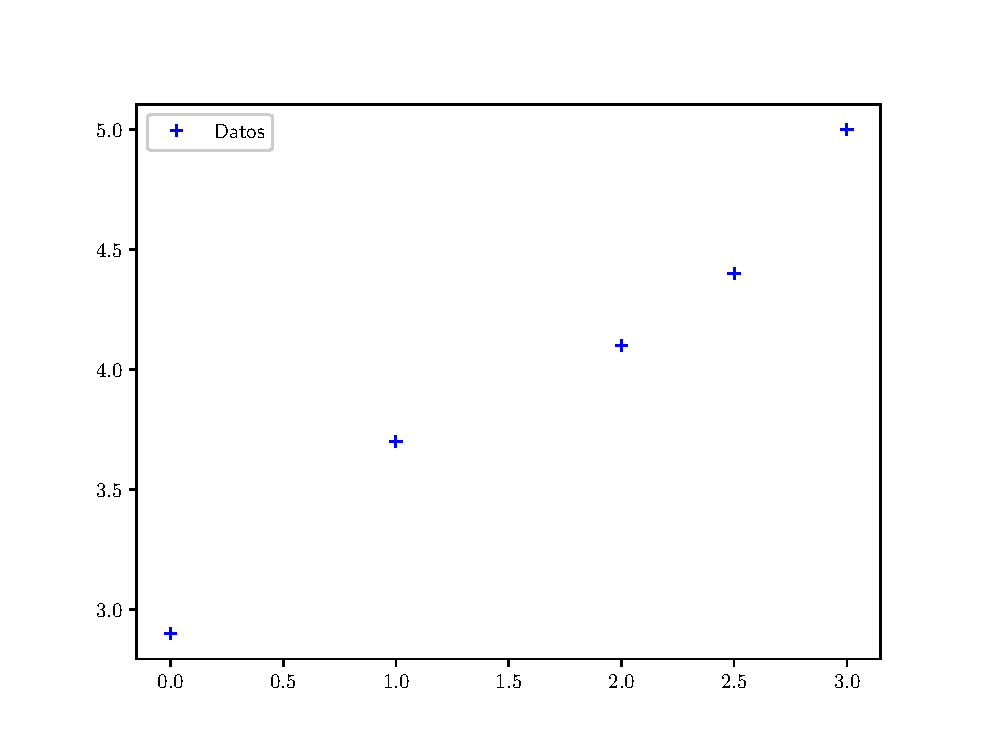
\includegraphics[scale=0.6]{Imagenes/Intro_Interpolacion_001.eps}
    %\caption{Tenemos un conjunto de datos experimentales obtenidos en el laboratorio.}
\end{figure}
\end{frame}
\begin{frame}[fragile]
\frametitle{Interpolación vs ajuste con curvas}
\begin{figure}
    \centering
    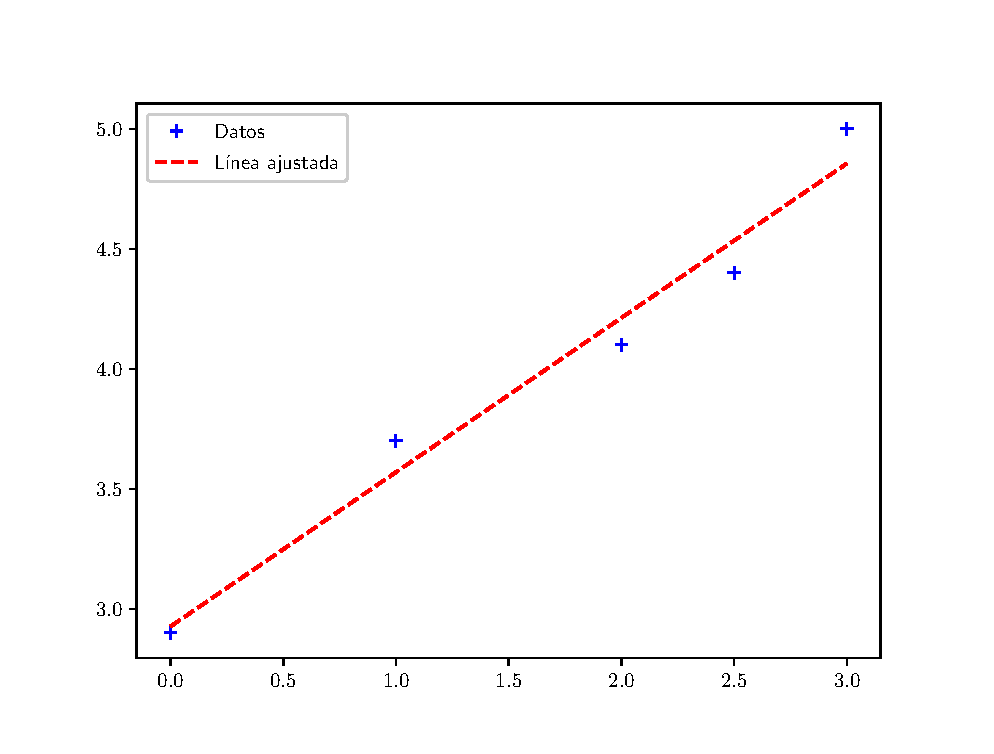
\includegraphics[scale=0.6]{Imagenes/Intro_Interpolacion_002.eps}
    %\caption{La técnica de ajuste de curvas es una aproximación al conjunto de datos.}
\end{figure}
\end{frame}
\begin{frame}[fragile]
\frametitle{Interpolación vs ajuste con curvas}
\begin{figure}
    \centering
    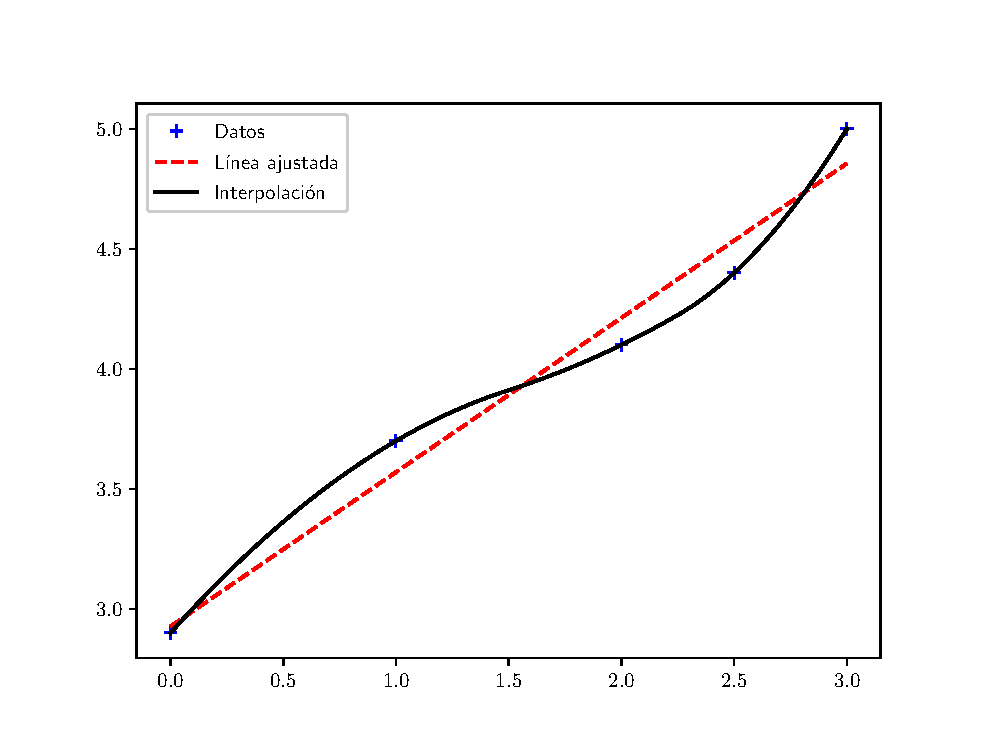
\includegraphics[scale=0.6]{Imagenes/Intro_Interpolacion_003.eps}
    %\caption{Con la interpolación se construye una curva suave que \enquote{toca} a los puntos experimentales.}
\end{figure}
\end{frame}

\subsection*{Ejemplos}

\begin{frame}
\frametitle{Determinar la vida media de un elemento}
Tomemos como ejemplo una fuente radioactiva y un detector, el cual contabiliza el número de decaimientos.
\\
\bigskip
\pause
Para determinar la vida media de la fuente, debemos de contar los decaimientos $N_{0}$, $N_{1}$, $N_{2}$, $\ldots$, $N_{k}$, en los tiempos $t_{0}$, $t_{1}$, $t_{2}$, $\ldots$, $t_{k}$
\end{frame}
\begin{frame}
\frametitle{Identificando la variable independiente}
En este ejemplo, \textcolor{red}{la variable independiente es $t$}, siendo la forma  apropiada para resolver el problema. 
\\
\bigskip
\pause
Sin embargo, tenemos un conjunto discreto de pares de números $(t_{k}, N_{k})$ en el rango de $(t_{0}, t_{k}$)
\end{frame}
\begin{frame}
\frametitle{Función que nos indique valores}
Con la intención de obtener información del experimento, deberíamos de encontrar una función analítica que nos devuelva el valor de $N$ para cualquier punto arbitrario $t$.
\end{frame}
\begin{frame}
\frametitle{Función que nos indique valores}
Pero a veces, el tratar de encontrar una función analítica es imposible, o el pensar en utilizar una función conocida, nos podría llevar mucho tiempo para calcularla, más si nuestro interés se basa en una pequeña vecindad de la variable independiente.
\end{frame}
\begin{frame}
\frametitle{El caso del americio}
Supongamos que tenemos una fuente radioactiva de {}$^{241}$Am, una fuente de rayos $\alpha$. Su vida media es $\tau_{\frac{1}{2}} = 430$ años.
\\
\bigskip
\pause
Obviamente no podríamos determinar su vida media midiéndola, ya que el decaimiento es lento y quizá lo que podríamos hacer es medir cada lunes durante algunos meses: después de cinco meses (por ejemplo) podríamos detener las mediciones y revisar los datos.
\end{frame}
\begin{frame}
\frametitle{Respondiendo una pregunta}
Una pregunta que nos podemos plantear es: ¿cuál fue la actividad el miércoles de la tercera semana de mediciones? 
\\
\bigskip
\pause
Ya que ese día está dentro del rango de mediciones $(t_{0}, t_{k})$
\end{frame}
\begin{frame}
\frametitle{La interpolación es una respuesta}
Lo que podríamos hacer es usar técnicas de \textcolor{blue}{interpolación} para determinar ese valor.  
\\
\bigskip
\pause
Si lo que queremos, es el caso contrario, conocer la actividad luego de ocho meses posteriores a la última medición, lo que deberíamos de hacer es \textcolor{red}{extrapolar} a ese punto a partir de las mediciones previas.
\end{frame}

\subsection{Objetivo de la interpolación}

\begin{frame}
\frametitle{Objetivo de la interpolación}
La idea central de la interpolación es seleccionar una función $g (x)$ tal que $g (x_{i}) = f_{i}$ para cada dato $i$, es una buena aproximación para cualquier otro dato $x$ entre el conjunto original de datos.
\end{frame}
\begin{frame}
\frametitle{Objetivo de la interpolación}
Pero ¿cómo podemos considerar una buena aproximación al conjunto de datos, si no tenemos la función original?
\\
\bigskip
\pause
Dado que los puntos ser pueden interpolar por una familia infinita de funciones, para ello debemos de contar con algún criterio o guía para seleccionar una función razonable.
\end{frame}
\begin{frame}
\frametitle{Criterio de suavidad al ajuste}
La regla para esos métodos se basa en la \textcolor{red}{suavidad al ajuste} de las funciones de interpolación.
\end{frame}
\begin{frame}
\frametitle{Criterio de suavidad al ajuste}
Pero esto no podría funcionar para todo tipo de funciones, consideremos la función:
\\
\medskip
\pause
\begin{minipage}{3cm}
\begin{align*}
g(x) = \dfrac{1}{25 \, x^{2}}
\end{align*}
\end{minipage}
\hspace{0.5cm}
\begin{minipage}{6cm}
\begin{figure}
	\centering
	 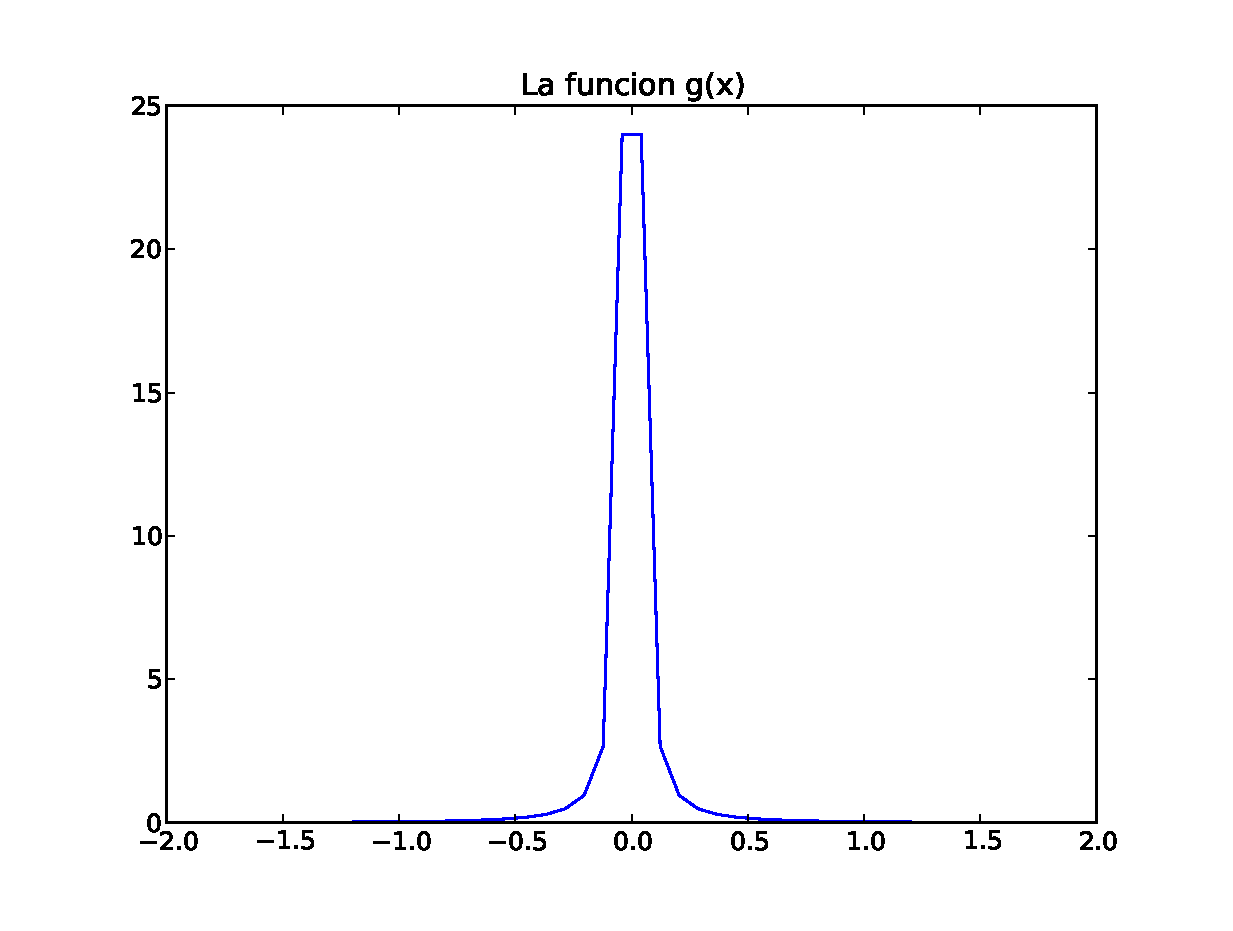
\includegraphics[scale=0.3]{Imagenes/grafica02.eps}  
\end{figure}
\end{minipage}
\end{frame}

\subsection{Consideración previa}

\begin{frame}
\frametitle{Consideración previa}
Antes de entrar de lleno a la revisión de las técnicas de interpolación, es necesario mencionar lo siguiente: dado que contamos con un conjunto finito de puntos, debemos de tener cuidado en el espaciamiento de la variable independiente.
\end{frame}
\begin{frame}
\frametitle{Consideración previa}
Si los puntos se alejan unos de otros, perderemos información para aquellos valores entre éstos puntos y la predicción de la interpolación ya no será la esperada.
\end{frame}
\begin{frame}
\frametitle{Ejemplo 3}
Supongamos que tenemos seis mediciones como se indican en la siguiente figura, podemos ver claramente un comportamiento oscilatorio de la función, juzgando por los puntos y de acuerdo a las barras de error, una línea recta es la que probablemente nos ajustaría los puntos.
\end{frame}
\begin{frame}
\frametitle{Ejemplo 3}
\begin{figure}
	\centering
	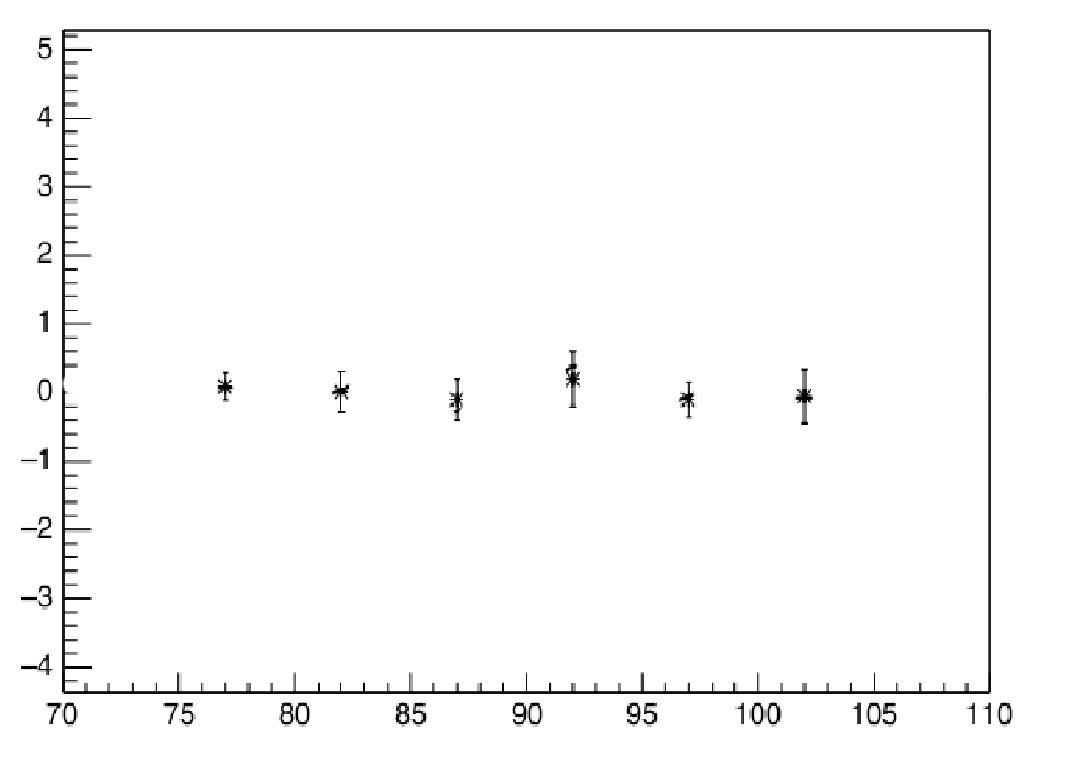
\includegraphics[scale=0.6]{Imagenes/figura01-1.eps} 
\end{figure}
\end{frame}
\begin{frame}
\frametitle{Gráfica de una interpolación}
Las técnicas de interpolación hacen lo que pidamos, pero no necesariamente son consistentes con un fenómeno o modelo.
\pause
\begin{figure}
	\centering
		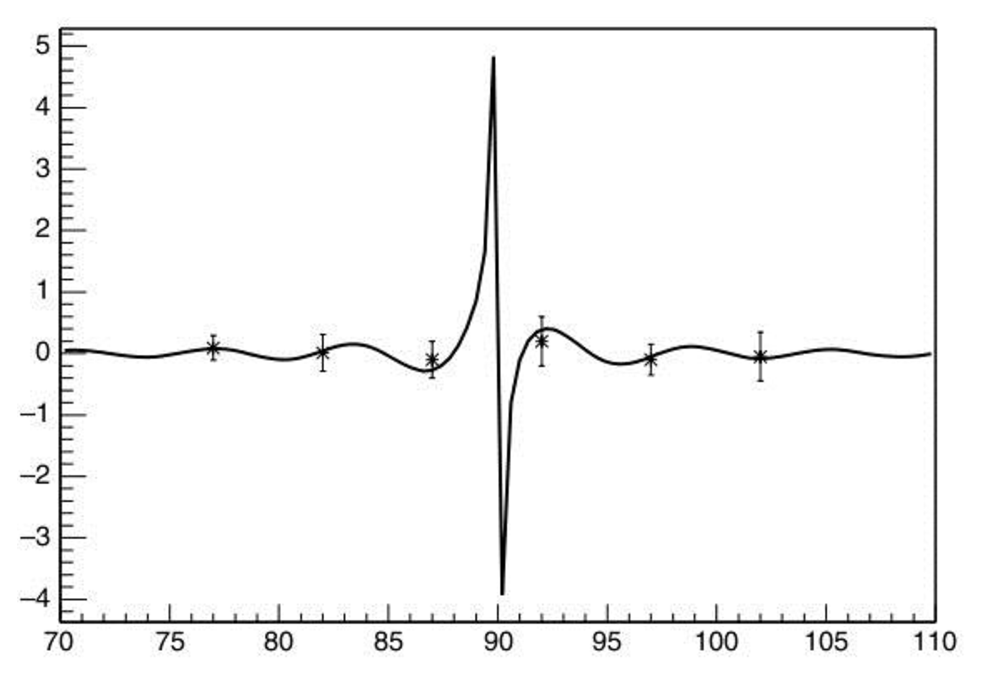
\includegraphics[scale=0.4]{Imagenes/figura02.eps} 
\end{figure}
\end{frame}

\section{Interpolación polinomial}
\frame{\tableofcontents[currentsection, hideothersubsections]}
\subsection{Interpolación de Lagrange}

\begin{frame}
\frametitle{Interpolación de Lagrange}
La técnica más sencilla de interpolación, es usando polinomios. \pause Siempre es posible construir un \emph{único} polinomio de grado $n$ que pasa a través de $n + 1$ puntos.
\\
\medskip
\pause
Una manera de obtener este polinomio es usando la fórmula de Lagrange.
\end{frame}
\begin{frame}
\frametitle{Fórmula de Lagrange}
\begin{equation}
P_{n} (x) = \nsum_{i = 0}^{n} \: y_{i} \: \ell_{i} (x)
\label{eq:ecuacion_03_01a}
\end{equation}
donde $n$ es el grado del polinomio y
\pause
\begin{align}
\begin{aligned}
\ell_{i} (x) &= \dfrac{x - x_{0}}{x_{i} - x_{0}} \cdot \dfrac{x - x_{1}}{x_{i} - x_{1}} \ldots \dfrac{x - x_{i + 1}}{x_{i} - x_{i + 1}} \cdot \dfrac{x - x_{n}}{x_{i} - x_{n}} \\
 &= \prod_{\substack{j = 0 \\ j \neq i}}^{n} \; \dfrac{x - x_{j}}{x_{i} - x_{j}}, \hspace{0.5cm} i = 0,1,\ldots,n
\end{aligned}
\label{eq:ecuacion_03_01b}
\end{align}
se llaman \emph{funciones cardinales}.
\end{frame}
\begin{frame}
\frametitle{Por ejemplo, si $n = 1$}
La interpolación es una línea recta:
\pause
\begin{align*}
P_{1} (x) = y_{0} \: \ell_{0} (x) + y_{1} \: \ell_{1} (x)
\end{align*}
y las funciones cardinales son:
\pause
\begin{align*}
\ell_{0} (x) = \dfrac{x - x_{1}}{x_{0} - x_{1}} \hspace{1cm} \ell_{1} (x) = \dfrac{x - x_{0}}{x_{1} - x_{0}}
\end{align*}
\end{frame}
\begin{frame}
\frametitle{Con $n = 2$}
La interpolación es parabólica:
\pause
\begin{align*}
P_{2} (x) = y_{0} \: \ell_{0} (x) + y_{1} \: \ell_{1} (x) + y_{2} \: \ell_{2} (x)
\end{align*}
y las $\mathcal{L}_{i}(x)$ son:
\begin{align*}
\ell_{0} (x) &= \dfrac{(x - x_{1})(x - x_{2})}{(x_{0} - x_{1})(x_{0} - x_{2})} \\
\ell_{1} (x) &= \dfrac{(x - x_{0})(x - x_{2})}{(x_{1} - x_{0})(x_{1} - x_{2})} \\
\ell_{2} (x) &= \dfrac{(x - x_{0})(x - x_{1})}{(x_{2} - x_{0})(x_{2} - x_{1})} 
\end{align*}
\end{frame}
\begin{frame}
\frametitle{Propiedad de las funciones cardinales}
Las funciones cardinales son polinomios de orden $n$ que tienen la propiedad:
\pause
\begin{align}
\ell_{i} (x_{j}) = \begin{cases} 0 \hspace{0.1cm} \mbox{si } i \neq j \\ 
1 \hspace{0.1cm} \mbox{si } i = j \end{cases} = \delta_{ij}
\label{eq:ecuacion_03_02}
\end{align}
donde $\delta_{ij}$ es la delta de Kronecker.
\end{frame}
\begin{frame}
\frametitle{Fórmula de Lagrange}
Para probar que el polinomio de interpolación pasa por los puntos experimentales, sustituimos $x = x_{j}$ en la definición de $P_{n} (x)$ (ec. \ref{eq:ecuacion_03_01a}) y usamos la ec. (\ref{eq:ecuacion_03_02}), entonces:
\pause
\begin{align*}
P_{n} (x_{j}) = \sum_{i = 0}^{n} y_{i} \: \ell_{i}(x_{j}) = \sum_{i = 0}^{n} y_{i} \: \delta_{ij} = y_{j}
\end{align*}
\end{frame}
\begin{frame}
\frametitle{Error en la fórmula de Lagrange}
Se puede demostrar que el error en el polinomio de interpolación es:
\pause
\begin{align*}
f(x) - P_{n} (x) = \dfrac{(x - x_{0})(x - x_{1}) \ldots (x - x_{n})}{(n + 1)!} \: f^{(n+1)} (\xi)
\end{align*}
donde $\xi \in (x_{0},x_{n})$, y éste valor normalmente no se conoce. 
\\
\bigskip
\pause
Debemos de notar que mientras más lejos están los datos de $x$, contribuye a que el error se incremente. 
\end{frame}

\subsubsection{Interpolando}

\begin{frame}
\frametitle{Ejercicio dei interpolación}
Veamos el cambio de la presión del vapor de {}$^{4}$He como función de la temperatura, de acuerdo a la literatura tenemos que:
\pause
\begin{center}
\renewcommand{\arraystretch}{0.9}
\begin{tabular}{c | l@{}}
Temperatura [K] & Presión de vapor [kPa] \\
\hline $2.3$ & $6.38512$ \\
\hline $2.7$ & $13.6218$ \\
\hline $2.9$ & $18.6760$ \\
\hline $3.2$ & $28.2599$ \\
\hline $3.5$ & $40.4082$ \\
\hline $3.7$ & $49.9945$
\end{tabular}
\end{center}
\end{frame}
\begin{frame}
\frametitle{Gráfica de los puntos experimentales}
\begin{figure}
	\centering
	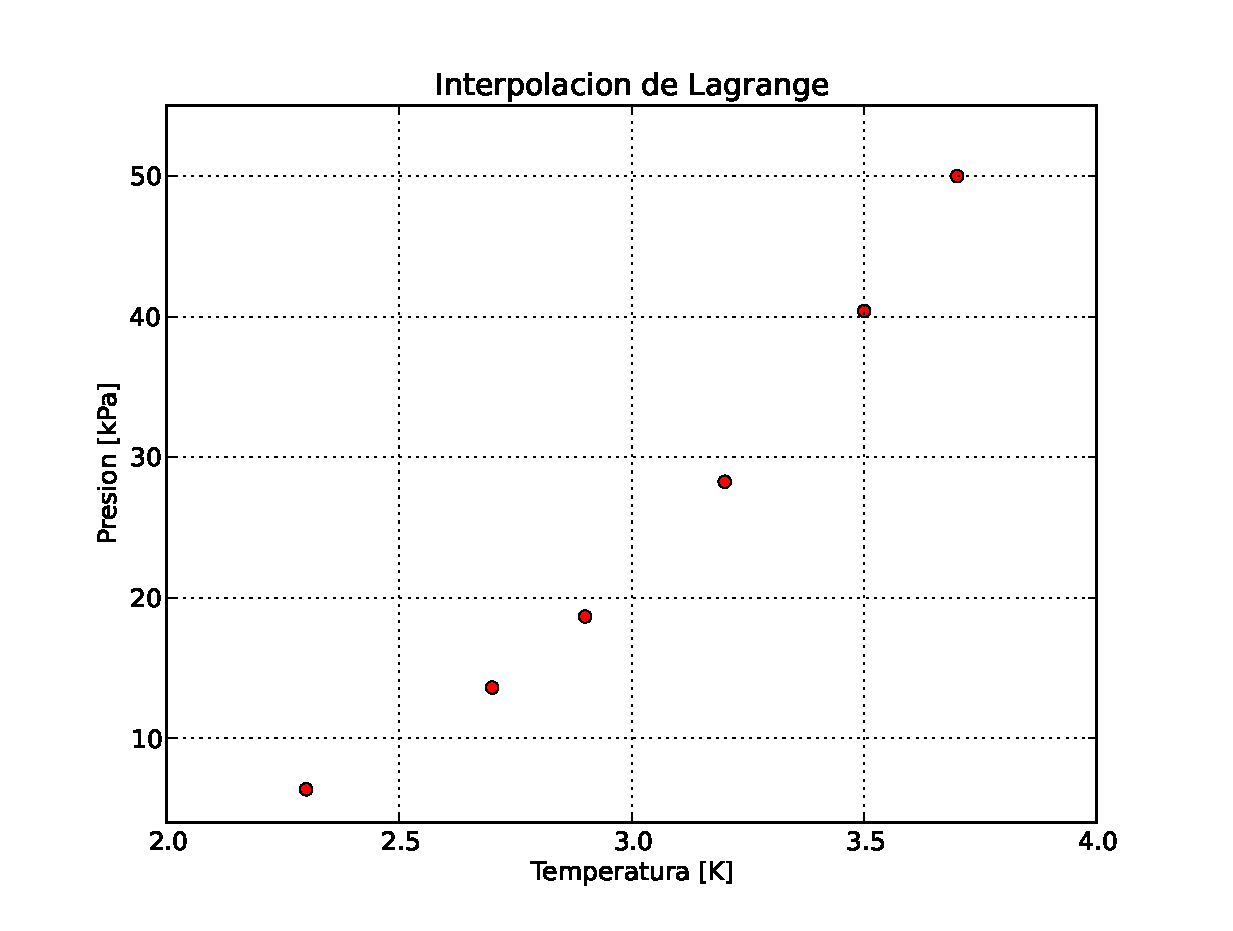
\includegraphics[scale=0.4]{Imagenes/grafica03_1.eps}
	\caption{El conjunto de datos experimentales.}
\end{figure}
\end{frame}
\begin{frame}
\frametitle{Pregunta para resolver}
¿Cuál es el valor de presión a una temperatura de $\SI{3}{\kelvin}$?
\begin{figure}
	\centering
	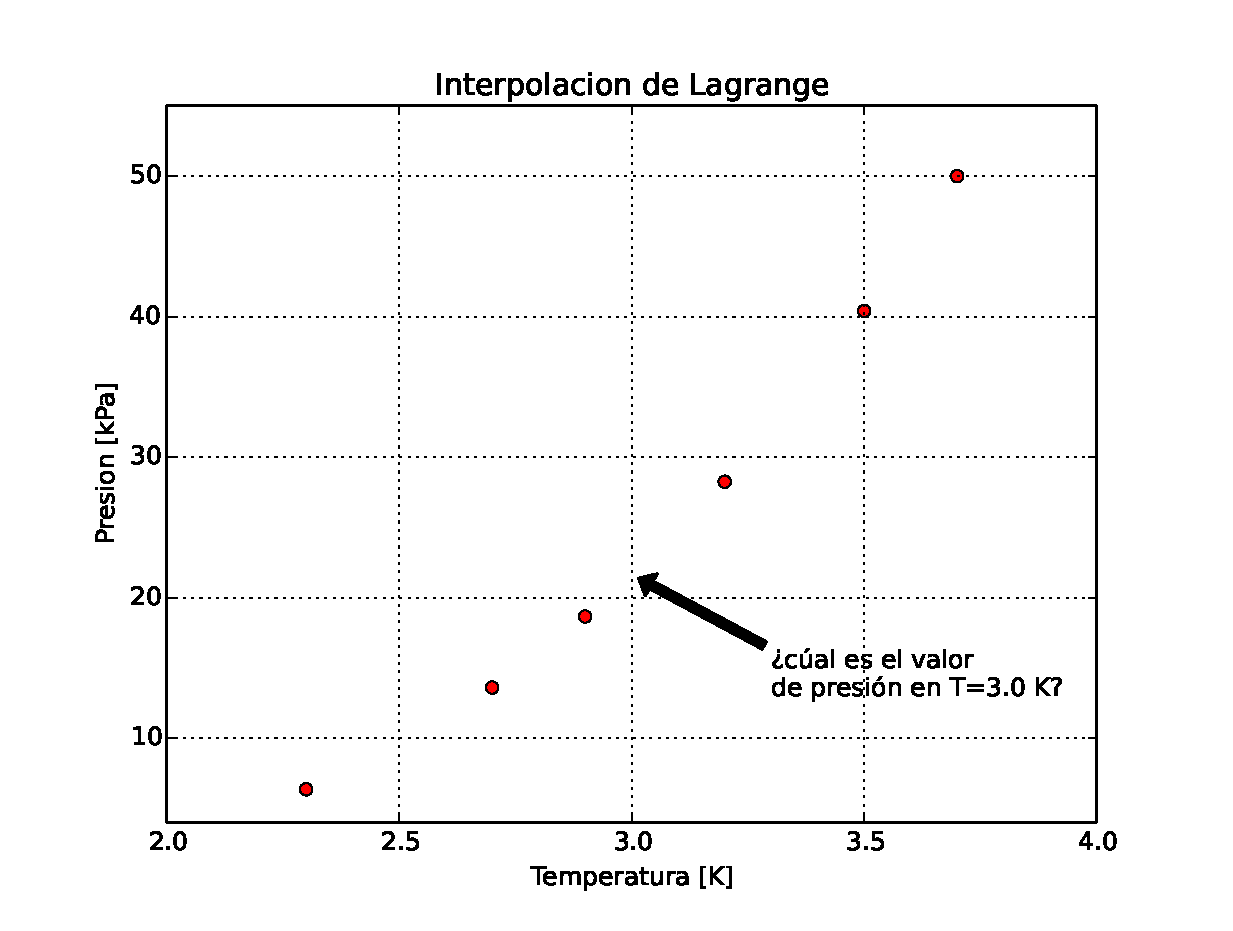
\includegraphics[scale=0.4]{Imagenes/grafica03.eps} 
\end{figure}
\end{frame}
\begin{frame}[fragile]
\frametitle{Solución}
Tomamos lo que ya conocemos para $n = 1$:
\pause
\begin{align*}
P_{1} (x) = y_{0} \: \ell_{0} (x) + y_{1} \: \ell{1} (x)
\end{align*}
\pause
y las funciones cardinales son:
\pause
\begin{align*}
\ell_{0} (x) = \dfrac{x - x_{1}}{x_{0} - x_{1}} \hspace{1cm} \ell_{1} (x) = \dfrac{x - x_{0}}{x_{1} - x_{0}}
\end{align*}
\end{frame}
\begin{frame}[fragile]
\frametitle{Solución}
En nuestro ejemplo, tenemos que:
\pause
\begin{align*}
(x_{0}, y_{0}) = (2.9, 18.6760) \\[1em]
(x_{1}, y_{1}) = (3.2, 28.2599)
\end{align*}
\pause
Con la interpolación lineal, tenemos que para una temperatura de \textcolor{blue}{$\SI{3.0}{\kelvin}$}, la presión tiene un valor de \textcolor{red}{$\mathbf{\SI{21.87}{\kilo\pascal}}$}
\end{frame}
\begin{frame}
\frametitle{Interpolación cuadrática}
Con la intención de mejorar nuestro resultado, podemos usar un polinomio de segundo orden, es decir $n = 2$:
\pause
\begin{align*}
P_{2} (x) = y_{0} \: \ell_{0} (x) + y_{1} \: \ell_{1} (x) + y_{2} \: \ell_{2} (x)
\end{align*}
\end{frame}
\begin{frame}
\frametitle{Interpolación cuadrática}
Las funciones cardinales $\ell_{i}(x)$ son:
\pause
\begin{align*}
\ell_{0} (x) &= \dfrac{(x - x_{1})(x - x_{2})}{(x_{0} - x_{1})(x_{0} - x_{2})} \\[1em]
\ell_{1} (x) &= \dfrac{(x - x_{0})(x - x_{2})}{(x_{1} - x_{0})(x_{1} - x_{2})} \\[1em]
\ell_{2} (x) &= \dfrac{(x - x_{0})(x - x_{1})}{(x_{2} - x_{0})(x_{2} - x_{1})} 
\end{align*}
\end{frame}
\begin{frame}
\frametitle{Usando los datos experimentales}
Usando los valores de la tabla anterior:
\pause
\begin{eqnarray*}
(x_{0}, y_{0}) = (2.7, 13.6218) \\
(x_{1}, y_{1}) = (2.9, 18.6760) \\
(x_{2}, y_{2}) = (3.2, 28.2599)
\end{eqnarray*}
\pause
A una temperatura de \textcolor{blue}{$\SI{3.0}{\kelvin}$}, la presión de vapor tiene un valor de \textcolor{red}{$\mathbf{\SI{21.671}{\kilo\pascal}}$}
\\
\bigskip
\visible<3->{El siguiente paso es usar cuatro puntos y construir el polinomio de orden $3$.}
\end{frame}
\begin{frame}
\frametitle{Ejercicio a cuenta}
Resuelve el ejercicio de interpolar con $4$ puntos de la tabla y obtén el valor de la presión de vapor a $\SI{3.0}{\kelvin}$.
\\
\bigskip
¿Cuál es la diferencia en el resultado al tomar distintos puntos de la tabla? Es decir, tomando $2$ puntos antes y después de los $\SI{3.0}{\kelvin}$, o tomando $3$ antes y $1$ punto después de los $\SI{3.0}{\kelvin}$, etc. Presenta una tabla con los valores. Usando \python{} te será más fácil los cálculos. 
\end{frame}

\end{document}